\documentclass[12pt]{article}
\usepackage{amsmath,amssymb,amsfonts}
\usepackage{geometry}
\usepackage{hyperref}
\geometry{a4paper, margin=1in}

\title{Unified Biquaternion Theory 2.0 (Consolidated)}
\author{David Jaroš}
\date{\today}

\begin{document}
\maketitle
\tableofcontents

\appendix

\section{Appendix A: Fine-Structure Constant in UBT — Topology, Precise Running, and Prime/$p$-Adic Multiplexing}
\label{app:alpha-consolidated}

\subsection{Topological origin: \(\alpha_0^{-1}=N\)}
We adopt the Chern quantization of the \(U(1)\) bundle (Appendix~\ref{app:adelic-holonomy}):
\begin{equation}
\frac{1}{2\pi}\int_{\Sigma} F = N \in \mathbb{Z}\,, \qquad \Rightarrow \qquad \alpha_0^{-1}=N\,.
\end{equation}
For the physical branch we take a prime, indecomposable class \(N=137\).

\subsection{Precise low-energy value via QED running}
Quantum vacuum polarization shifts \(\alpha\) according to one-loop QED
\begin{equation}
\alpha^{-1}(\mu) = N + \frac{1}{3\pi}\ln\!\frac{m_e^2}{\mu^2} \;(+\;\text{thresholds and higher orders})\,.
\end{equation}
With \(N=137\) this is satisfied by \(\mu/m_e \approx 0.84397\), consistent with the internal-mode scale of the UBT electron solution.
Higher-order and threshold terms can be included in the standard way without altering the topological identification of \(N\).

\subsection{Prime/$p$-adic multiplexing (optional hypothesis)}
As a conservative extension (see Appendix~\ref{app:padic-prelim}), one can regard prime \(N\) as a discrete ``channel'' labeling independent
theta-modes of the complex-time torus. This suggests a family of prime branches with
\begin{equation}
\alpha_0^{-1}=N\,, \quad N\in\mathbb{P}\,,
\end{equation}
where nearby primes (e.g. \(131, 139\)) give universes similar to ours after the same QED running. The $p$-adic layer
provides a natural arithmetic underpinning of the prime preference; we keep it as an interpretive add-on without changing the
core derivation above.

\section{Appendix B: Electromagnetism in UBT — Classical, Emergent, and Geometric Views}
% TODO: merge all EM texts here as subsections: classical Maxwell sector, emergent-current derivation, KK embedding.

\section{Appendix C: Lepton Mass Hierarchy from Internal Modes}
% TODO: reconstruct electron internal-mode derivation and extend to muon/tau.


\section{Appendix E: Standard Model Coupling and QCD Embedding in UBT}
\label{app:sm-qcd-ubt}

\subsection{Overview}
This appendix restores and consolidates the linkage between the Unified Biquaternion Theory (UBT) and the
Standard Model (SM) gauge structure, with special emphasis on the QCD sector. We present a consistent dictionary
from the UBT geometric variables to the SM gauge potentials and field strengths, and we state matching conditions
and running-coupling relations compatible with Appendices~\ref{app:alpha-consolidated} and \ref{app:padic-rigorous}.

\subsection{Gauge bundle and connections}
Let the SM gauge group be
\[
\mathbb{G} \;\cong\; SU(3)_c \times SU(2)_L \times U(1)_Y\,.
\]
We introduce gauge connections (one-forms) and field strengths:
\begin{align}
G_\mu &\;=\; G_\mu^a T^a \in \mathfrak{su}(3), &
G_{\mu\nu} &= \partial_\mu G_\nu - \partial_\nu G_\mu + i g_s\,[G_\mu, G_\nu], \\
W_\mu &\;=\; W_\mu^i \tau^i \in \mathfrak{su}(2), &
W_{\mu\nu} &= \partial_\mu W_\nu - \partial_\nu W_\mu + i g\,[W_\mu, W_\nu], \\
B_\mu &\in \mathfrak{u}(1), &
B_{\mu\nu} &= \partial_\mu B_\nu - \partial_\nu B_\mu.
\end{align}
The covariant derivative acting on a matter field $\Psi$ in a representation $(\mathbf{3},\mathbf{2},Y)$ reads
\begin{equation}
D_\mu \Psi \;=\; \Big(\partial_\mu + i g_s G_\mu^a T^a + i g W_\mu^i \tau^i + i g^\prime Y B_\mu\Big)\Psi.
\end{equation}

\subsection{UBT $\to$ SM dictionary}
UBT provides a unified connection $\mathcal{A}_\mu$ on the $\psi$-fibered spacetime. We assume a block-diagonal projection
\begin{equation}
\mathcal{A}_\mu \;\longmapsto\; (G_\mu,\, W_\mu,\, B_\mu)
\end{equation}
such that the $U(1)$ normalization is fixed by the Chern quantization as in Appendix~\ref{app:alpha-consolidated}.
The electric charge operator obeys $Q = T^3 + Y/2$, and the electroweak mixing is
\begin{equation}
\begin{pmatrix} A_\mu \\ Z_\mu \end{pmatrix} \;=\;
\begin{pmatrix} \cos\theta_W & \sin\theta_W \\ -\sin\theta_W & \cos\theta_W \end{pmatrix}
\begin{pmatrix} B_\mu \\ W^3_\mu \end{pmatrix},
\qquad
e \;=\; g \sin\theta_W \;=\; g^\prime \cos\theta_W.
\end{equation}
At low energies $e$ matches $\alpha$ derived in Appendix~\ref{app:alpha-consolidated}. The determination of $\theta_W$ and $(g,g^\prime)$
requires additional matching conditions (left for future work) or a unification hypothesis.

\subsection{Gauge-invariant Lagrangian}
The gauge kinetic terms are
\begin{equation}
\mathcal{L}_{\rm gauge} \;=\; -\frac{1}{4}\,G_{\mu\nu}^a G^{a\,\mu\nu} \;-\; \frac{1}{4}\,W_{\mu\nu}^i W^{i\,\mu\nu} \;-\; \frac{1}{4}\,B_{\mu\nu} B^{\mu\nu}.
\end{equation}
For QCD with $n_f$ quark flavors the matter part includes
\begin{equation}
\mathcal{L}_{\rm QCD}^{\rm matter} \;=\; \sum_{f=1}^{n_f} \bar{q}_f\,(i\gamma^\mu D_\mu - m_f)\,q_f\,,
\qquad D_\mu q \;=\; (\partial_\mu + i g_s G_\mu^a T^a)q.
\end{equation}

\subsection{Running couplings and matching}
\paragraph{QED.} The low-energy fine-structure constant $\alpha(\mu)$ is fixed by the UBT topological integer $N$ and
vacuum polarization as in Appendix~\ref{app:alpha-consolidated}.

\paragraph{QCD.} The strong coupling runs according to
\begin{equation}
\alpha_s(\mu) \;=\; \frac{g_s^2(\mu)}{4\pi} \;=\; \frac{1}{\beta_0 \ln(\mu^2/\Lambda_{\rm QCD}^2)}\Big(1 - \frac{\beta_1}{\beta_0^2}\frac{\ln\ln(\mu^2/\Lambda^2_{\rm QCD})}{\ln(\mu^2/\Lambda^2_{\rm QCD})} + \cdots\Big),
\end{equation}
with $\beta_0=\tfrac{11}{4\pi}\!-\!\tfrac{n_f}{6\pi}$ and $\beta_1=\tfrac{102}{(4\pi)^2}\!-\!\tfrac{38\,n_f}{(4\pi)^2}$ in the $\overline{\rm MS}$ scheme. Asymptotic freedom ($\beta_0>0$) and confinement at low $\mu$ are consistent with a knotted-flux interpretation in the $\Theta$ sector.

\subsection{Topological interpretation of QCD in UBT}
Color flux tubes correspond to knotted configurations of $\Theta$ with nontrivial linking.
Wilson loops $\langle \mathrm{Tr}\, \mathcal{P}\exp i\oint G\rangle$ map to holonomies of $\mathcal{A}_\mu$ in the UBT fiber;
an area law for large loops is compatible with an energy cost proportional to knotted tube length and curvature.
Instanton sectors ($\pi_3(SU(2))\cong \mathbb{Z}$) mirror Hopf-like textures, providing a common topological language for both EM and QCD sectors.

\subsection{Matching conditions and open tasks}
\begin{itemize}
\item \textbf{Normalization:} $U(1)$ is fixed by Chern quantization (Appendix~\ref{app:alpha-consolidated}). The QCD normalization is anchored by $\Lambda_{\rm QCD}$; in UBT one expects $\Lambda_{\rm QCD}\sim \xi\,\mu_{\rm int}$, with the internal-mode scale $\mu_{\rm int}$ from the electron sector and $\xi=\mathcal{O}(1)$ to be fitted.
\item \textbf{Electroweak mixing:} determining $\theta_W$ from UBT requires an additional symmetry or a unification hypothesis; otherwise it is an independent parameter.
\item \textbf{Anomalies:} the SM matter assignment must satisfy anomaly cancellation; UBT embeddings should preserve this (check fermion content mapping).
\item \textbf{Hadron phenomenology:} flux-tube/knotted-state spectra vs.\ lattice-QCD input is an avenue for quantitative tests.
\end{itemize}

\subsection{Consistency with dark matter appendix}
The interaction portals between the $\Theta$ topological sector and colored matter are suppressed by orthogonality (complex-time fiber)
and higher-dimensional operators. Therefore QCD does not spoil the DM stability discussed in Appendix~\ref{app:dm-consolidated}, while gravitational coupling remains universal.

================================================================================\appendix{G}{Dark Matter as Topological Excitations in $\Theta(q,\tau)$ Field}

\section{Introduction}
In the Unified Biquaternion Theory (UBT), dark matter (DM) emerges naturally as a set of topologically protected excitations in the fundamental $\Theta(q,\tau)$ field, where $q$ are the biquaternionic coordinates and $\tau = t + i\psi$ is the complex time. The theory identifies these excitations with \emph{hopfions}, knotted field configurations classified by the Hopf index $Q_H \in \mathbb{Z}$, which are stable due to topological constraints.

\section{Relation to Baryonic Matter and Pseudospin States}
While baryonic matter corresponds to localized, symmetry-broken excitations with strong coupling to the $SU(3) \times SU(2) \times U(1)$ gauge fields, dark matter modes occupy orthogonal pseudospin sectors of $\Theta(q,\tau)$.
The $\psi$ (imaginary time) component effectively decouples them from direct gauge interactions in our visible sector. This explains why dark matter interacts only gravitationally and via higher-order topological couplings.

Let $\Theta = (\theta_1, \theta_2, ..., \theta_N)$ denote the components of the field in an $SU(2)$ pseudospin basis. Baryonic matter resides in subspaces with $\psi \approx 0$, whereas DM modes have $\psi \neq 0$, leading to an effective suppression factor
\begin{equation}
g_{\mathrm{eff}} \sim e^{-\frac{\psi^2}{\psi_0^2}},
\end{equation}
where $\psi_0$ is a characteristic phase scale.

\section{Weak Interaction Mechanism}
The suppression factor above follows from integrating out the orthogonal modes in the path integral formulation of UBT. The leading-order interaction term between DM hopfions and baryons has the schematic form:
\begin{equation}
\mathcal{L}_{\mathrm{int}} \sim \frac{\lambda_{\mathrm{top}}}{M_{\mathrm{Pl}}^2} \, J_{\mathrm{baryon}}^\mu J_{\mathrm{DM},\mu},
\end{equation}
where $\lambda_{\mathrm{top}}$ is a dimensionless topological coupling constant, $J_{\mathrm{baryon}}^\mu$ is the baryonic current, and $J_{\mathrm{DM}}^\mu$ is the dark matter topological current. The Planck-scale suppression explains the extreme weakness of the interaction.

\section{Energy Density Calculation}
Let the spectrum of DM topological modes be indexed by $n$, with each mode having an energy
\begin{equation}
E_n = \hbar \omega_0 \sqrt{n^2 + \alpha Q_H^2},
\end{equation}
where $\alpha$ is a coupling constant between the mode number and the Hopf index.

Assuming a thermal-like distribution in the early universe with an effective temperature $T_{\mathrm{DM}}$, the energy density becomes
\begin{equation}
\rho_{\mathrm{DM}} = \frac{1}{V} \sum_{n,Q_H} g_{n,Q_H} \, E_n \, e^{-E_n/k_B T_{\mathrm{DM}}}.
\end{equation}
For a continuous approximation and $T_{\mathrm{DM}} \ll \hbar\omega_0$, the integral yields
\begin{equation}
\rho_{\mathrm{DM}} \approx \frac{g_{\mathrm{eff}} \, (\hbar\omega_0)^{5/2}}{(2\pi)^{3/2}} \, e^{-\hbar\omega_0/k_B T_{\mathrm{DM}}}.
\end{equation}
Matching to Planck satellite cosmological measurements $\rho_{\mathrm{DM}}/\rho_{\mathrm{crit}} \approx 0.265$ allows extraction of $\omega_0$ or $g_{\mathrm{eff}}$ in terms of fundamental UBT parameters.

\section{Experimental Detection in UBT Framework}
A possible detection method involves modulating the phase $\psi$ in a toroidal $\Theta$-resonator, tuned to frequencies corresponding to $\omega_0$ of the DM spectrum. The coupling is expected to produce minute phase shifts or sideband structures in the resonator's electromagnetic response.

\subsection{Dark Photons and $p$-adic Extension}
In the $p$-adic extension of UBT, each prime $p$ defines an independent $\Theta_p(q,\tau)$ sector. In some universes, the dominant DM component may correspond to $p$-adic photons (``dark photons''), which are massless gauge bosons in the $\Theta_p$ sector, invisible to our $p= \infty$ (real-number) sector except via gravity or suppressed topological mixing.

The mixing Lagrangian can be schematically written as:
\begin{equation}
\mathcal{L}_{\mathrm{mix}} \sim \epsilon_{p} F^{\mu\nu}(\Theta_{\infty}) F_{\mu\nu}(\Theta_p),
\end{equation}
where $\epsilon_{p} \ll 1$ is the $p$-dependent kinetic mixing parameter.

\section{Conclusion}
The UBT description of dark matter as hopfions and other topological modes in $\Theta(q,\tau)$ provides a unified explanation for its stability, weak interactions, and observed abundance. The inclusion of $p$-adic sectors opens a pathway for describing alternate-reality DM components such as dark photons, potentially accessible through precision topological resonance experiments.

\section{Appendix G: Dark Matter in UBT --- Topological Solitons, Quantum Corrections, and Prime/$p$-Adic Sectors}
\label{app:dm-consolidated}

\subsection{Scope and Motivation}
This appendix consolidates all dark-matter (DM) content relevant to UBT~2.0 into a single, rigorous narrative.
It unifies: (i) topological solitons (Hopfions and knotted configurations) of the $\Theta(q,\tau)$ field,
(ii) quantum corrections around those backgrounds, (iii) hidden prime/$p$-adic sectors producing gravitationally coupled but electromagnetically silent components,
and (iv) phenomenology and constraints.

\subsection{Topological Sector of the $\Theta$ Field}
Let $\Theta:\mathbb{R}^3\!\to\!S^2$ be the (unit) phase map obtained after $U(1)$ gauge-fixing from the UBT order parameter.
Compactifying $\mathbb{R}^3\cup\{\infty\}\cong S^3$, homotopy classes $[S^3,S^2]$ are labeled by the Hopf invariant $Q_H\in\mathbb{Z}$.
A standard energy functional supporting static Hopf solitons is
\begin{equation}
\label{eq:ubt-hopf-energy}
E[\Theta] \;=\; \int d^3x \Big\{ \frac{\kappa_2}{2}\,\partial_i\Theta\!\cdot\!\partial_i\Theta \;+\; \frac{\kappa_4}{4}\,\big(\partial_i\Theta\times\partial_j\Theta\big)^2 \Big\}\,,
\end{equation}
with $\kappa_{2,4}>0$ effective couplings inherited from the UBT Lagrangian. The Hopf charge admits
\begin{equation}
Q_H \;=\; \frac{1}{32\pi^2}\int d^3x\,\epsilon^{ijk}\,\mathcal{A}_i\,\mathcal{F}_{jk}\,,\qquad
\mathcal{F}_{ij}=\partial_i\mathcal{A}_j-\partial_j\mathcal{A}_i,\quad
\partial_i\Theta=\mathcal{F}_{ij}\times \Theta,
\end{equation}
and is conserved under smooth time evolution. Minimizers at fixed $Q_H$ are knotted/linked tubes of field lines (Hopfions).
The classical scaling bound $E \ge c\,|Q_H|^{3/4}$ (Vakulenko--Kapitanski) applies for \eqref{eq:ubt-hopf-energy} under mild hypotheses.

\paragraph{Size and mass scales.}
Balancing the quadratic and quartic terms gives a characteristic radius $R_H\sim(\kappa_4/\kappa_2)^{1/2}$ and a mass scale
\begin{equation}
M_H \;\sim\; \frac{1}{c^2}\,\frac{\kappa_2^{3/2}}{\kappa_4^{1/2}}\ \mathcal{C}\,|Q_H|^{3/4}\,,\qquad \mathcal{C}=\mathcal{O}(1).
\end{equation}
Within UBT, $\kappa_{2,4}$ trace back to the same normalization that fixes the electromagnetic coupling (Appendix~\ref{app:alpha-consolidated})
and are therefore not arbitrary.

\subsection{Complex Time and Phase-Linked Hopfions}
The UBT substrate uses $\tau=t+i\psi$. Allow the soliton profile to depend on $\psi$ through a phase-linked ansatz
\begin{equation}
\Theta(x,t,\psi) \;=\; \Theta_{\rm cl}(x;\lambda(\psi))\,,
\end{equation}
with slow $\psi$-modulation of moduli $\lambda$ obeying an effective geodesic law in moduli space.
This generates a small internal mode that remains gapped provided the Skyrme term stabilizes the core.
The imaginary-time modulation is responsible for the exponential suppression of non-topological decays.

\subsection{Quantum Fluctuations (One-Loop Correction)}
Expand $\Theta=\Theta_{\rm cl}+\delta\Theta$ with $\delta\Theta\perp \Theta_{\rm cl}$. Quadratic fluctuations yield
\begin{equation}
S^{(2)}[\delta\Theta] \;=\; \frac{1}{2}\int d^4x\, \delta\Theta\,\hat{\mathcal{O}}[\Theta_{\rm cl}]\,\delta\Theta\,,
\end{equation}
where $\hat{\mathcal{O}}$ is positive and gapped on $S^3$ after compactification.
The one-loop mass shift is
\begin{equation}
\Delta M_{H}^{\rm 1\text{-}loop} \;=\; \frac{\hbar}{2c^2}\,\mathrm{Tr}\Big(\sqrt{\hat{\mathcal{O}}}-\sqrt{\hat{\mathcal{O}}_0}\Big)\,,
\end{equation}
and the physical mass $M_H^{\rm phys}=M_H+\Delta M_H^{\rm 1\text{-}loop}+\cdots$.
In UBT, the cutoff and counterterms are linked to the internal-mode scale which also controls the low-energy renormalization of $\alpha$,
ensuring consistent scale setting across sectors.

\subsection{Production and Relic Abundance}
Hopfions are naturally produced non-thermally during symmetry-breaking or topological phase transitions.
Treat them as nonrelativistic quasiparticles with dispersion $E_k\simeq M_H^{\rm phys}c^2 + k^2/(2M_H^{\rm phys})$.
The comoving density $n_H$ satisfies
\begin{equation}
\frac{dn_H}{dt}+3H n_H \;=\; \mathcal{S}_{\rm topo}(T)\;-\;\langle\sigma v\rangle_{\rm unlink}\, n_H^2 \;+\; \cdots,
\end{equation}
where $\mathcal{S}_{\rm topo}$ encodes nonthermal production by defect formation and $\langle\sigma v\rangle_{\rm unlink}$ is exponentially suppressed by the core size and fluctuation gap.
The present-day energy density is
\begin{equation}
\rho_{\rm DM}^{\rm (Hopf)} \;=\; \int \frac{d^3k}{(2\pi)^3}\, f_H(k)\, E_k
\;\simeq\; n_H\, M_H^{\rm phys}c^2\,,
\end{equation}
with $f_H$ set by the formation history. Quantum corrections only renormalize $M_H$ and thus $\rho_{\rm DM}$ multiplicatively.

\subsection{Electromagnetic Silence and Interaction Portals}
Direct electromagnetic couplings are suppressed by phase orthogonality: the Hopfion core lives in the $\Theta$ sector orthogonal to the visible $U(1)$ phase.
Allowed portals are: (i) gravitational, (ii) higher-derivative curvature couplings, and (iii) extremely weak mixing through multi-$\Theta$ operators consistent with UBT symmetries.
These are naturally below existing direct-detection limits if $\hat{\mathcal{O}}$ remains gapped and $R_H$ is not microscopic.

\subsection{Prime/$p$-Adic Hidden Sectors}
The adelic extension (Appendix~\ref{app:padic-rigorous}) yields prime-indexed sectors $\Theta_p$ satisfying
\begin{equation}
\langle \Theta_p,\Theta_q\rangle \;=\; 0 \quad (p\neq q)\,,
\end{equation}
by orthogonality of characters and CRT factorization.
Each prime branch $p$ can host its own Hopfion population with mass $M_H^{(p)}$ and cross section $(\sigma/m)_p$.
The total DM is a sum over branches
\begin{equation}
\rho_{\rm DM}^{\rm total} \;=\; \sum_{p\in\mathcal{P}^\star}\rho_{\rm DM}^{(p)} \,,
\end{equation}
with $\mathcal{P}^\star$ a finite set in the truncated adele. As branches couple only gravitationally at low energies, they evade thermalization with the visible sector, preserving standard cosmology.

\subsection{Astrophysical and Cosmological Signatures}
\textbf{Halo structure.} Finite $R_H$ induces cored profiles at small radii; superposition of branches can emulate multi-component halos.
\textbf{Lensing.} DM acts as pressureless dust at large scales; substructure from knotted domains can induce small lensing anomalies.
\textbf{Indirect detection.} Radiative decays are topologically forbidden; unlinking annihilations are exponentially suppressed $\sim e^{-R_H\,\Delta}$.
\textbf{Direct detection.} Nuclear scattering via higher-derivative portals is naturally below current bounds for $R_H\!\gtrsim\!{\rm fm}$ and small mixing.

\subsection{Consistency with the Electromagnetic Sector}
The same UBT normalization that fixes the $U(1)$ sector and the fine-structure constant (Appendix~\ref{app:alpha-consolidated}) also sets $\kappa_{2,4}$ and the fluctuation gap in \eqref{eq:ubt-hopf-energy}.
Hence $M_H$ and the derived $\rho_{\rm DM}$ co-vary with the internal-mode scale, tying DM and EM predictions to a common geometric origin.

\subsection{Minimal Parameter Inference (Practical Template)}
Given an observational target $(\rho_{\rm DM}, \sigma/m)$ and a chosen prime set $\mathcal{P}^\star$, the following steps infer UBT parameters:
\begin{enumerate}
\item Fix the internal-mode scale from the $\alpha$ analysis (Appendix~\ref{app:alpha-consolidated}).
\item Choose $Q_H$ and solve the classical soliton for $(\kappa_2,\kappa_4)$ with $R_H\!\sim\!(\kappa_4/\kappa_2)^{1/2}$.
\item Compute $\hat{\mathcal{O}}$ on $S^3$ and evaluate $\Delta M_H^{\rm 1\text{-}loop}$ (heat-kernel or phase-shift methods).
\item Evolve $n_H$ with a nonthermal source $\mathcal{S}_{\rm topo}(T)$; check CMB/BBN and structure-formation constraints.
\item If including prime sectors, repeat for each $p\in\mathcal{P}^\star$ and sum $\rho_{\rm DM}^{(p)}$.
\end{enumerate}

\subsection{Summary}
UBT provides two robust DM mechanisms grounded in its geometry: (i) topologically protected Hopfions of the $\Theta$ field, dressed by controlled quantum corrections, and (ii) orthogonal prime/$p$-adic sectors with their own cold components.
Both are gravitationally coupled and naturally compatible with cosmological bounds. Their mass and interaction scales are linked to the same internal-mode physics that fixes $\alpha$, yielding correlated predictions across sectors.

\appendix{G: Dark Matter as Topological Hopfions in Unified Biquaternion Theory}

\section*{Introduction}
In the Unified Biquaternion Theory (UBT), dark matter is modeled as topologically stable field configurations – \emph{hopfions} – arising as non-trivial mappings between compactified spatial slices \(S^3\) and internal field space \(S^2\). These configurations are solutions to the UBT field equations for the tensor–spinor field \(\Theta(q,\tau)\) with non-zero Hopf invariant \(Q_H \in \mathbb{Z}\).

Unlike conventional particle dark matter candidates (e.g., WIMPs, axions), hopfions do not require direct coupling to the Standard Model fields; their stability is protected by topological conservation laws.

\section*{Mathematical Formulation}
Let the UBT field \(\Theta: S^3 \to S^2\) be expressed in normalized complex components \(\Theta = (\phi_1, \phi_2) \in \mathbb{C}^2\), satisfying \(|\phi_1|^2 + |\phi_2|^2 = 1\). The Hopf invariant is defined as:

\begin{equation}
Q_H = \frac{1}{(4\pi)^2} \int_{S^3} \mathbf{A} \wedge \mathbf{F},
\end{equation}
where \(\mathbf{F} = d\mathbf{A}\) is the field strength associated with the pullback of the area form on \(S^2\).

The energy functional in the biquaternionic Lagrangian takes the form:
\begin{equation}
E[\Theta] = \int_{\mathbb{R}^3} \left( \alpha |\nabla \Theta|^2 + \beta |\mathbf{F}|^2 \right) \, d^3x,
\end{equation}
with \(\alpha, \beta\) determined by the underlying UBT coupling constants.

\section*{Hopfion Solutions and Stability}
Minimization of \(E[\Theta]\) under fixed \(Q_H\) yields knotted soliton solutions. In the UBT framework, these solutions are generalized to include the complex-time coordinate \(\tau = t + i\psi\), giving rise to \emph{phase–linked hopfions} where the imaginary time \(\psi\) modulates their internal twist.

Stability is guaranteed by the integer-valued Hopf invariant; any continuous deformation preserving field smoothness cannot change \(Q_H\).

\section*{Dark Matter Interpretation}
Hopfions interact only gravitationally and through topology–mediated phase effects with normal matter. Their contribution to the energy–momentum tensor in the UBT metric is given by:
\begin{equation}
T_{\mu\nu}^{\text{hopfion}} = 2\alpha \partial_\mu \Theta \cdot \partial_\nu \Theta^* + 2\beta F_{\mu\lambda} F_{\nu}{}^\lambda - g_{\mu\nu} \mathcal{L}_{\text{hopfion}}.
\end{equation}

Cosmologically, a relic density of hopfions could arise naturally during symmetry-breaking phase transitions in the early Universe, analogously to cosmic strings or monopoles, but without leading to observational inconsistencies thanks to their low interaction cross-section.

\section*{Observational Signatures}
Possible observational consequences include:
\begin{itemize}
\item Microlensing events without electromagnetic counterparts.
\item Non-Gaussian features in the CMB due to large-scale hopfion structures.
\item Anomalous gravitational wave dispersion from hopfion–induced metric perturbations.
\end{itemize}

\section*{Conclusion}
The UBT hopfion model provides a purely topological candidate for dark matter, naturally arising from the field \(\Theta(q,\tau)\) without introducing ad hoc particles. This aligns with the theory’s aim to unify physical phenomena through a single geometric–algebraic framework.

\section*{Appendix G: Dark Matter, Hopfions, and Topological Excitations in the $\Theta$-Field}
\addcontentsline{toc}{section}{Appendix G: Dark Matter, Hopfions, and Topological Excitations in the $\Theta$-Field}
\subsection*{G.1 Motivation}
Within the Unified Biquaternion Theory (UBT), the master field $\Theta(q,\tau)$ allows for nontrivial topological configurations. 
A particularly relevant class are \emph{Hopfions}---localized, finite-energy field configurations characterized by a nonzero Hopf invariant. 
We outline their mathematical structure, dynamics in complex time $\tau=t+i\psi$, energetic properties, and gravitational phenomenology as candidates for (a component of) dark matter.
\subsection*{G.2 Hopf Map and Topological Index}
The canonical Hopf fibration maps $S^3 \to S^2$. 
Introduce a complex doublet $z=(z_1,z_2)^T\in\mathbb{C}^2$ with $z^\dagger z = 1$ (so that $z$ parametrizes $S^3$). 
The unit vector $n:\mathbb{R}^3\cup\{\infty\}\simeq S^3 \to S^2$ is
n^a = z^\dagger \sigma^a z,\qquad a=1,2,3,
where $\sigma^a$ are the Pauli matrices. The $U(1)$ connection and curvature are
A_i = -i\, z^\dagger \partial_i z,\qquad F_{ij} = \partial_i A_j - \partial_j A_i.
The \emph{Hopf invariant} is
Q_H \;=\; \frac{1}{4\pi^2}\int_{\mathbb{R}^3} \mathrm{d}^3x\; \epsilon^{ijk}\, A_i F_{jk} \;\in\; \mathbb{Z},
which counts the linking number of preimages in $n(\mathbf{x})$. Finite-energy boundary conditions compactify space to $S^3$, ensuring $Q_H$ is topological.
\subsection*{G.3 Biquaternionic Representation}
In UBT, the $\Theta$-field takes values in the biquaternion algebra $\mathbb{B}$. 
A minimal embedding of a Hopfion uses a normalized doublet $z(q,\tau)$ extracted from $\Theta(q,\tau)$ through a projection $\Pi:\mathbb{B}\to\mathbb{C}^2$:
z(q,\tau) \;=\; \Pi\!\left[\Theta(q,\tau)\right],\qquad z^\dagger z = 1.
The physical $n(q,\tau)$ and the $U(1)$ potential $A_i(q,\tau)$ then follow from the above constructions, with possible $\psi$-dependence via $\tau=t+i\psi$.
\subsection*{G.4 Energetics and the Faddeev--Skyrme Functional}
A standard energy functional supporting stable Hopfions is the Faddeev--Skyrme model:
E[n] \;=\; \int\! \mathrm{d}^3x \;\Big\{ \alpha\, (\partial_i n)^2 \;+\; \beta\, (F_{ij})^2 \Big\},\qquad n\cdot n=1.
In our setting, $\alpha,\beta$ can acquire a weak $\psi$-dependence from the complex-time sector,
\alpha \to \alpha(\psi),\qquad \beta \to \beta(\psi),
and additional small corrections may arise from couplings to electromagnetic and matter fields (Appendix D, F). 
The topological lower bound scales as $E \gtrsim c\, |Q_H|^{3/4}$ for some constant $c>0$, consistent with known Hopfion energy--charge relations.
\subsection*{G.5 Dynamics in Complex Time}
Allowing slow $\psi$-evolution, the effective Lagrangian density reads
\mathcal{L}_{\mathrm{Hopf}} \;=\; \frac{1}{2} \kappa_\psi \, (\partial_\psi n)^2 \;+\; \frac{1}{2}\rho \, (\partial_t n)^2 \;-\; \alpha(\psi)\, (\partial_i n)^2 \;-\; \beta(\psi)\, (F_{ij})^2 \;-\; V(n;\psi),
with $V$ encoding weak explicit symmetry breaking or environmental pinning. 
Variations give a generalized Landau--Lifshitz-type equation with a Skyrme term and small $\psi$-derivative corrections, stabilizing knotted textures under perturbations:
\rho\, \partial_t^2 n + \kappa_\psi\, \partial_\psi^2 n \;-\; 2\,\alpha \,\Delta n \;+\; \cdots \;=\; \lambda(x,\psi,t)\, n,\qquad n\cdot n=1.
\subsection*{G.6 Gravitational Coupling and Dark-Matter Phenomenology}
Coupling to gravity proceeds via the stress--energy tensor derived from $\mathcal{L}_{\mathrm{Hopf}}$:
T_{\mu\nu} \;=\; \frac{\partial \mathcal{L}}{\partial(\partial^\mu n)}\cdot \partial_\nu n \;-\; g_{\mu\nu}\,\mathcal{L},
supplemented by contributions from the $\psi$-sector. 
In galactic halos, an ensemble of dilute, long-lived Hopfions with typical size $R_H$ and charge $Q_H=\mathcal{O}(1\text{--}10)$ yields an effective mass density
\rho_{\mathrm{DM}} \;\approx\; \frac{N_H\, E(Q_H)}{V_{\mathrm{halo}}} \;\sim\; \frac{N_H}{V_{\mathrm{halo}}}\, c\, |Q_H|^{3/4},
where $N_H$ is the number of Hopfions in volume $V_{\mathrm{halo}}$. 
Since Hopfions are neutral in the $U(1)$ electromagnetic sector (projection to $A_\mu$ vanishes at infinity) and interact mainly through gravity (and possibly very weak $\psi$-mediated channels), they are natural dark-matter candidates in UBT.
\subsection*{G.7 Couplings to Electromagnetism and Matter}
At low energies, allowed gauge-invariant couplings are suppressed by small parameters:
\mathcal{L}_{\mathrm{int}} \;=\; - g_{nA}\, ( \partial_i n \cdot \partial_j n )\, F^{ij} \;-\; g_{nF}\, (F_{ij})^2\, ( \partial_k n )^2 \;-\; g_{n\psi}\, (\partial_\psi n)^2\, \bar{\Psi}\Psi \;+\; \cdots,
leading to minute birefringence-like effects or dispersion shifts (Appendix D) only in extreme conditions. 
Psychon-induced $\psi$-fluctuations (Appendix F) may modulate Hopfion stability via $\kappa_\psi$ and $\beta(\psi)$, offering a route to small, structured signatures without spoiling standard-model tests.
\subsection*{G.8 3D Schematic: Linked Flux Surfaces (Hopf Link)}
\begin{figure}[h!]
\centering
\tdplotsetmaincoords{70}{120}
\begin{tikzpicture}[tdplot_main_coords,scale=1.0, line cap=round,line join=round]
  % Parameters for two linked circles (Hopf link)
  \def\R{2.2}
  \def\r{0.9}
  % Circle 1 in x-y plane
  \draw[very thick, blue!70!black]
    plot[domain=0:360, samples=200, variable=\t]
    ({\R*cos(\t)}, {\R*sin(\t)}, {0});
  % Circle 2 in x-z plane, shifted to link with circle 1
  \draw[very thick, red!70!black]
    plot[domain=0:360, samples=200, variable=\u]
    ({0}, {\r*cos(\u)}, {\r*sin(\u)});
  % Soft field-line hints
  \foreach \k in {0,30,...,330}{
    \draw[blue!40!black, opacity=0.35]
      plot[domain=0:360, samples=80, variable=\t]
      ({(\R+0.3*cos(\k))*cos(\t)}, {(\R+0.3*cos(\k))*sin(\t)}, {0.2*sin(\k)});
  }
  \node[anchor=south] at (0,-2.9,0) {\small Schematic Hopf link representing linked preimages of $n(\mathbf{x})$ (topological charge $Q_H=1$)};
\end{tikzpicture}
\caption{Conceptual 3D schematic of a Hopfion as a linked flux structure (Hopf link).}
\label{fig:hopf_link}
\end{figure}
\subsection*{G.9 Observational and Experimental Windows}
\item \textbf{Astrophysics:} core/halo profiles modified by a population of stable knotted excitations; lensing and rotation curve fits with effective pressure terms from Skyrme corrections.
\item \textbf{Cosmology:} early-universe production of Hopfions during symmetry-breaking transitions; relic abundance depending on $\alpha(\psi),\beta(\psi)$.
\item \textbf{Laboratory analogues:} knotted light and superfluid vortices as table-top proxies to test relaxation/stability scaling.
\subsection*{G.10 Summary and Open Questions}
Hopfions provide a topologically protected, electromagnetically neutral sector consistent with UBT and compatible with precision QED. 
Key open directions include: quantitative halo modeling with $\psi$-dependent parameters, production mechanisms in cosmology, and refined bounds on weak couplings to standard fields.
\subsection*{G.11 Explicit $Q_H=1$ Parametrization (Stereographic Construction)}
Let $r^2=x^2+y^2+z^2$. A standard explicit $S^3\!\to\!S^2$ Hopf-map representative (unit charge $Q_H=1$) can be written via a normalized doublet $z=(z_1,z_2)^T$,
z(\mathbf{x}) \;=\; \frac{1}{r^2+1}\begin{pmatrix}
(r^2-1) + 2 i z \\[4pt]
2(x+i y)
\end{pmatrix},\qquad z^\dagger z = 1.
Then
n^a(\mathbf{x}) = z^\dagger(\mathbf{x})\,\sigma^a\, z(\mathbf{x}),\qquad
A_i(\mathbf{x})=-i\, z^\dagger \partial_i z,\qquad F_{ij}=\partial_i A_j-\partial_j A_i,
and the Hopf invariant
Q_H \;=\; \frac{1}{4\pi^2}\int\!\mathrm{d}^3x\;\epsilon^{ijk} A_i F_{jk} \;=\; 1.
A size (core-radius) parameter $R_0$ is introduced by the replacement $\mathbf{x}\mapsto \mathbf{x}/R_0$ in $z(\mathbf{x})$, which scales the configuration without changing $Q_H$.
\paragraph{Biquaternion Embedding.} In UBT one may take $z=\Pi[\Theta]$ for a projection $\Pi:\mathbb{B}\!\to\!\mathbb{C}^2$; the above $z(\mathbf{x})$ fixes the $\Theta$ phase-texture up to internal rotations, preserving $Q_H=1$ in the projected $U(1)$ sector.
\subsection*{G.12 Order-of-Magnitude Estimates (Size, Energy, Density)}
For the Faddeev--Skyrme energy functional
E[n] \;=\; \int\!\mathrm{d}^3x\;\Big\{\alpha\, (\partial_i n)^2 + \beta\, (F_{ij})^2\Big\},
Derrick scaling with $n(\mathbf{x})\to n(\lambda \mathbf{x})$ yields
E(\lambda)= \alpha\, \lambda\, I_2 + \beta\, \lambda^{-1} I_4,\qquad
I_2=\!\int\! (\partial_i n)^2,\ \ I_4=\!\int\! (F_{ij})^2,
minimized at $\lambda_\star=\sqrt{\dfrac{\beta I_4}{\alpha I_2}}$ with
E_{\min}=2\sqrt{\alpha\beta\, I_2 I_4},\qquad
R_H \;\propto\; \lambda_\star^{-1} \;\sim\; \sqrt{\frac{\beta}{\alpha}}\, \Big(\frac{I_2}{I_4}\Big)^{1/4}.
For $Q_H=1$ one typically has $I_2,I_4=\mathcal{O}(1)$ (dimensionless after extracting a core scale), hence the \emph{size--energy} scalings
R_H \sim \sqrt{\frac{\beta}{\alpha}},\qquad E_{Q=1} \sim \kappa\, \sqrt{\alpha\beta},
with $\kappa=\mathcal{O}(1)$ depending on the specific profile. For general charge $Q_H$, numerical studies give $E \gtrsim c\,|Q_H|^{3/4}$; a practical interpolation is
E(Q_H)\ \approx\ \kappa\, \sqrt{\alpha\beta}\, |Q_H|^{3/4}.
\paragraph{Illustrative Density.} For an ensemble of $N_H$ Hopfions of typical size $R_H$ (non-overlapping) in a halo volume $V_{\rm halo}$,
\rho_{\rm DM} \;\approx\; \frac{N_H\, E(Q_H)}{V_{\rm halo}} \ \sim\  \frac{N_H}{V_{\rm halo}}\ \kappa\, \sqrt{\alpha\beta}\, |Q_H|^{3/4},
while kinematics and stability are controlled by $R_H\!\sim\!\sqrt{\beta/\alpha}$. The $\psi$-sector induces mild running $\alpha(\psi),\beta(\psi)$, enabling environmental dependence without spoiling topological protection.
\subsection*{G.13 Numerical Illustration (Order-of-Magnitude)}
To make the scaling relations concrete, consider illustrative (dimensionally normalized) parameters
\alpha = 2.0,\qquad \beta = 0.5,\qquad Q_H=1,\qquad \kappa \approx 1.
Then
R_H \sim \sqrt{\frac{\beta}{\alpha}} \;=\; \sqrt{\frac{0.5}{2.0}} \;\approx\; 0.5,\qquad
E_{Q=1} \sim \kappa\,\sqrt{\alpha\beta} \;=\; \sqrt{2.0\times 0.5} \;\approx\; 1.0.
For a sparse ensemble in a fiducial volume $V_{\rm halo}$ with number $N_H$,
\rho_{\rm DM} \;\approx\; \frac{N_H\,E_{Q=1}}{V_{\rm halo}} \;\approx\; \frac{N_H}{V_{\rm halo}}.
These values serve only as a \emph{scaling} guide; in physical units, $\alpha,\beta$ inherit dimensions from the microscopic UBT action and may acquire weak $\psi$-dependence, $\alpha(\psi),\beta(\psi)$, which shifts $R_H$ and $E$.

\appendix
\section*{Appendix G: Dark Matter, Hopfions, and Topological Excitations in the $\Theta$-Field}
\addcontentsline{toc}{section}{Appendix G: Dark Matter, Hopfions, and Topological Excitations in the $\Theta$-Field}

\subsection*{G.1 Motivation}
Within the Unified Biquaternion Theory (UBT), the master field $\Theta(q,\tau)$ allows for nontrivial topological configurations. 
A particularly relevant class are \emph{Hopfions}---localized, finite-energy field configurations characterized by a nonzero Hopf invariant. 
We outline their mathematical structure, dynamics in complex time $\tau=t+i\psi$, energetic properties, and gravitational phenomenology as candidates for (a component of) dark matter.

\subsection*{G.2 Hopf Map and Topological Index}
The canonical Hopf fibration maps $S^3 \to S^2$. 
Introduce a complex doublet $z=(z_1,z_2)^T\in\mathbb{C}^2$ with $z^\dagger z = 1$ (so that $z$ parametrizes $S^3$). 
The unit vector $n:\mathbb{R}^3\cup\{\infty\}\simeq S^3 \to S^2$ is
\begin{equation}
n^a = z^\dagger \sigma^a z,\qquad a=1,2,3,
\end{equation}
where $\sigma^a$ are the Pauli matrices. The $U(1)$ connection and curvature are
\begin{equation}
A_i = -i\, z^\dagger \partial_i z,\qquad F_{ij} = \partial_i A_j - \partial_j A_i.
\end{equation}
The \emph{Hopf invariant} is
\begin{equation}
Q_H \;=\; \frac{1}{4\pi^2}\int_{\mathbb{R}^3} \mathrm{d}^3x\; \epsilon^{ijk}\, A_i F_{jk} \;\in\; \mathbb{Z},
\end{equation}
which counts the linking number of preimages in $n(\mathbf{x})$. Finite-energy boundary conditions compactify space to $S^3$, ensuring $Q_H$ is topological.

\subsection*{G.3 Biquaternionic Representation}
In UBT, the $\Theta$-field takes values in the biquaternion algebra $\mathbb{B}$. 
A minimal embedding of a Hopfion uses a normalized doublet $z(q,\tau)$ extracted from $\Theta(q,\tau)$ through a projection $\Pi:\mathbb{B}\to\mathbb{C}^2$:
\begin{equation}
z(q,\tau) \;=\; \Pi\!\left[\Theta(q,\tau)\right],\qquad z^\dagger z = 1.
\end{equation}
The physical $n(q,\tau)$ and the $U(1)$ potential $A_i(q,\tau)$ then follow from the above constructions, with possible $\psi$-dependence via $\tau=t+i\psi$.

\subsection*{G.4 Energetics and the Faddeev--Skyrme Functional}
A standard energy functional supporting stable Hopfions is the Faddeev--Skyrme model:
\begin{equation}
E[n] \;=\; \int\! \mathrm{d}^3x \;\Big\{ \alpha\, (\partial_i n)^2 \;+\; \beta\, (F_{ij})^2 \Big\},\qquad n\cdot n=1.
\end{equation}
In our setting, $\alpha,\beta$ can acquire a weak $\psi$-dependence from the complex-time sector,
\begin{equation}
\alpha \to \alpha(\psi),\qquad \beta \to \beta(\psi),
\end{equation}
and additional small corrections may arise from couplings to electromagnetic and matter fields (Appendix D, F). 
The topological lower bound scales as $E \gtrsim c\, |Q_H|^{3/4}$ for some constant $c>0$, consistent with known Hopfion energy--charge relations.

\subsection*{G.5 Dynamics in Complex Time}
Allowing slow $\psi$-evolution, the effective Lagrangian density reads
\begin{equation}
\mathcal{L}_{\mathrm{Hopf}} \;=\; \frac{1}{2} \kappa_\psi \, (\partial_\psi n)^2 \;+\; \frac{1}{2}\rho \, (\partial_t n)^2 \;-\; \alpha(\psi)\, (\partial_i n)^2 \;-\; \beta(\psi)\, (F_{ij})^2 \;-\; V(n;\psi),
\end{equation}
with $V$ encoding weak explicit symmetry breaking or environmental pinning. 
Variations give a generalized Landau--Lifshitz-type equation with a Skyrme term and small $\psi$-derivative corrections, stabilizing knotted textures under perturbations:
\begin{equation}
\rho\, \partial_t^2 n + \kappa_\psi\, \partial_\psi^2 n \;-\; 2\,\alpha \,\Delta n \;+\; \cdots \;=\; \lambda(x,\psi,t)\, n,\qquad n\cdot n=1.
\end{equation}

\subsection*{G.6 Gravitational Coupling and Dark-Matter Phenomenology}
Coupling to gravity proceeds via the stress--energy tensor derived from $\mathcal{L}_{\mathrm{Hopf}}$:
\begin{equation}
T_{\mu\nu} \;=\; \frac{\partial \mathcal{L}}{\partial(\partial^\mu n)}\cdot \partial_\nu n \;-\; g_{\mu\nu}\,\mathcal{L},
\end{equation}
supplemented by contributions from the $\psi$-sector. 
In galactic halos, an ensemble of dilute, long-lived Hopfions with typical size $R_H$ and charge $Q_H=\mathcal{O}(1\text{--}10)$ yields an effective mass density
\begin{equation}
\rho_{\mathrm{DM}} \;\approx\; \frac{N_H\, E(Q_H)}{V_{\mathrm{halo}}} \;\sim\; \frac{N_H}{V_{\mathrm{halo}}}\, c\, |Q_H|^{3/4},
\end{equation}
where $N_H$ is the number of Hopfions in volume $V_{\mathrm{halo}}$. 
Since Hopfions are neutral in the $U(1)$ electromagnetic sector (projection to $A_\mu$ vanishes at infinity) and interact mainly through gravity (and possibly very weak $\psi$-mediated channels), they are natural dark-matter candidates in UBT.

\subsection*{G.7 Couplings to Electromagnetism and Matter}
At low energies, allowed gauge-invariant couplings are suppressed by small parameters:
\begin{equation}
\mathcal{L}_{\mathrm{int}} \;=\; - g_{nA}\, ( \partial_i n \cdot \partial_j n )\, F^{ij} \;-\; g_{nF}\, (F_{ij})^2\, ( \partial_k n )^2 \;-\; g_{n\psi}\, (\partial_\psi n)^2\, \bar{\Psi}\Psi \;+\; \cdots,
\end{equation}
leading to minute birefringence-like effects or dispersion shifts (Appendix D) only in extreme conditions. 
Psychon-induced $\psi$-fluctuations (Appendix F) may modulate Hopfion stability via $\kappa_\psi$ and $\beta(\psi)$, offering a route to small, structured signatures without spoiling standard-model tests.

\subsection*{G.8 3D Schematic: Linked Flux Surfaces (Hopf Link)}
\begin{figure}[h!]
\centering
\tdplotsetmaincoords{70}{120}
\begin{tikzpicture}[tdplot_main_coords,scale=1.0, line cap=round,line join=round]
  % Parameters for two linked circles (Hopf link)
  \def\R{2.2}
  \def\r{0.9}

  % Circle 1 in x-y plane
  \draw[very thick, blue!70!black]
    plot[domain=0:360, samples=200, variable=\t]
    ({\R*cos(\t)}, {\R*sin(\t)}, {0});

  % Circle 2 in x-z plane, shifted to link with circle 1
  \draw[very thick, red!70!black]
    plot[domain=0:360, samples=200, variable=\u]
    ({0}, {\r*cos(\u)}, {\r*sin(\u)});

  % Soft field-line hints
  \foreach \k in {0,30,...,330}{
    \draw[blue!40!black, opacity=0.35]
      plot[domain=0:360, samples=80, variable=\t]
      ({(\R+0.3*cos(\k))*cos(\t)}, {(\R+0.3*cos(\k))*sin(\t)}, {0.2*sin(\k)});
  }

  \node[anchor=south] at (0,-2.9,0) {\small Schematic Hopf link representing linked preimages of $n(\mathbf{x})$ (topological charge $Q_H=1$)};
\end{tikzpicture}
\caption{Conceptual 3D schematic of a Hopfion as a linked flux structure (Hopf link).}
\label{fig:hopf_link}
\end{figure}

\subsection*{G.9 Observational and Experimental Windows}
\begin{itemize}
\item \textbf{Astrophysics:} core/halo profiles modified by a population of stable knotted excitations; lensing and rotation curve fits with effective pressure terms from Skyrme corrections.
\item \textbf{Cosmology:} early-universe production of Hopfions during symmetry-breaking transitions; relic abundance depending on $\alpha(\psi),\beta(\psi)$.
\item \textbf{Laboratory analogues:} knotted light and superfluid vortices as table-top proxies to test relaxation/stability scaling.
\end{itemize}

\subsection*{G.10 Summary and Open Questions}
Hopfions provide a topologically protected, electromagnetically neutral sector consistent with UBT and compatible with precision QED. 
Key open directions include: quantitative halo modeling with $\psi$-dependent parameters, production mechanisms in cosmology, and refined bounds on weak couplings to standard fields.

\subsection*{G.11 Explicit $Q_H=1$ Parametrization (Stereographic Construction)}
Let $r^2=x^2+y^2+z^2$. A standard explicit $S^3\!\to\!S^2$ Hopf-map representative (unit charge $Q_H=1$) can be written via a normalized doublet $z=(z_1,z_2)^T$,
\begin{equation}
z(\mathbf{x}) \;=\; \frac{1}{r^2+1}\begin{pmatrix}
(r^2-1) + 2 i z \\[4pt]
2(x+i y)
\end{pmatrix},\qquad z^\dagger z = 1.
\end{equation}
Then
\begin{equation}
n^a(\mathbf{x}) = z^\dagger(\mathbf{x})\,\sigma^a\, z(\mathbf{x}),\qquad
A_i(\mathbf{x})=-i\, z^\dagger \partial_i z,\qquad F_{ij}=\partial_i A_j-\partial_j A_i,
\end{equation}
and the Hopf invariant
\begin{equation}
Q_H \;=\; \frac{1}{4\pi^2}\int\!\mathrm{d}^3x\;\epsilon^{ijk} A_i F_{jk} \;=\; 1.
\end{equation}
A size (core-radius) parameter $R_0$ is introduced by the replacement $\mathbf{x}\mapsto \mathbf{x}/R_0$ in $z(\mathbf{x})$, which scales the configuration without changing $Q_H$.

\paragraph{Biquaternion Embedding.} In UBT one may take $z=\Pi[\Theta]$ for a projection $\Pi:\mathbb{B}\!\to\!\mathbb{C}^2$; the above $z(\mathbf{x})$ fixes the $\Theta$ phase-texture up to internal rotations, preserving $Q_H=1$ in the projected $U(1)$ sector.

\subsection*{G.12 Order-of-Magnitude Estimates (Size, Energy, Density)}
For the Faddeev--Skyrme energy functional
\begin{equation}
E[n] \;=\; \int\!\mathrm{d}^3x\;\Big\{\alpha\, (\partial_i n)^2 + \beta\, (F_{ij})^2\Big\},
\end{equation}
Derrick scaling with $n(\mathbf{x})\to n(\lambda \mathbf{x})$ yields
\begin{equation}
E(\lambda)= \alpha\, \lambda\, I_2 + \beta\, \lambda^{-1} I_4,\qquad
I_2=\!\int\! (\partial_i n)^2,\ \ I_4=\!\int\! (F_{ij})^2,
\end{equation}
minimized at $\lambda_\star=\sqrt{\dfrac{\beta I_4}{\alpha I_2}}$ with
\begin{equation}
E_{\min}=2\sqrt{\alpha\beta\, I_2 I_4},\qquad
R_H \;\propto\; \lambda_\star^{-1} \;\sim\; \sqrt{\frac{\beta}{\alpha}}\, \Big(\frac{I_2}{I_4}\Big)^{1/4}.
\end{equation}
For $Q_H=1$ one typically has $I_2,I_4=\mathcal{O}(1)$ (dimensionless after extracting a core scale), hence the \emph{size--energy} scalings
\begin{equation}
R_H \sim \sqrt{\frac{\beta}{\alpha}},\qquad E_{Q=1} \sim \kappa\, \sqrt{\alpha\beta},
\end{equation}
with $\kappa=\mathcal{O}(1)$ depending on the specific profile. For general charge $Q_H$, numerical studies give $E \gtrsim c\,|Q_H|^{3/4}$; a practical interpolation is
\begin{equation}
E(Q_H)\ \approx\ \kappa\, \sqrt{\alpha\beta}\, |Q_H|^{3/4}.
\end{equation}
\paragraph{Illustrative Density.} For an ensemble of $N_H$ Hopfions of typical size $R_H$ (non-overlapping) in a halo volume $V_{\rm halo}$,
\begin{equation}
\rho_{\rm DM} \;\approx\; \frac{N_H\, E(Q_H)}{V_{\rm halo}} \ \sim\  \frac{N_H}{V_{\rm halo}}\ \kappa\, \sqrt{\alpha\beta}\, |Q_H|^{3/4},
\end{equation}
while kinematics and stability are controlled by $R_H\!\sim\!\sqrt{\beta/\alpha}$. The $\psi$-sector induces mild running $\alpha(\psi),\beta(\psi)$, enabling environmental dependence without spoiling topological protection.

\subsection*{G.13 Numerical Illustration (Order-of-Magnitude)}
To make the scaling relations concrete, consider illustrative (dimensionally normalized) parameters
\begin{equation}
\alpha = 2.0,\qquad \beta = 0.5,\qquad Q_H=1,\qquad \kappa \approx 1.
\end{equation}
Then
\begin{equation}
R_H \sim \sqrt{\frac{\beta}{\alpha}} \;=\; \sqrt{\frac{0.5}{2.0}} \;\approx\; 0.5,\qquad
E_{Q=1} \sim \kappa\,\sqrt{\alpha\beta} \;=\; \sqrt{2.0\times 0.5} \;\approx\; 1.0.
\end{equation}
For a sparse ensemble in a fiducial volume $V_{\rm halo}$ with number $N_H$,
\begin{equation}
\rho_{\rm DM} \;\approx\; \frac{N_H\,E_{Q=1}}{V_{\rm halo}} \;\approx\; \frac{N_H}{V_{\rm halo}}.
\end{equation}
These values serve only as a \emph{scaling} guide; in physical units, $\alpha,\beta$ inherit dimensions from the microscopic UBT action and may acquire weak $\psi$-dependence, $\alpha(\psi),\beta(\psi)$, which shifts $R_H$ and $E$.

% Appendix 11: Topological Modes and the Geometric Origin of Dark Matter
\documentclass[12pt]{article}
\usepackage{amsmath,amssymb,graphicx,geometry}
\geometry{margin=1in}
\title{Appendix 11: Topological Modes and the Geometric Origin of Dark Matter}
\author{Unified Biquaternion Theory Project}
\date{\today}

\begin{document}

\maketitle

\section*{Abstract}
We present a theoretical framework within the Unified Biquaternion Theory (UBT) in which dark matter arises naturally from topologically stable, electromagnetically neutral configurations of the fundamental field \( \Theta(q, \tau) \) in complexified spacetime \( \mathbb{C}^4 \). These configurations, termed "dark modes," carry gravitational mass-energy without electromagnetic interactions and are protected by the topological properties of the field.

\section{Topological Dark Modes}
Let the unified field \( \Theta(q, \tau) \) be defined over a complexified 4-manifold \( \mathbb{C}^4 \), where \( q \in \mathbb{C}^4 \) and \( \tau = t + i\psi \) is complex time. We define a dark mode \( \Theta_D \) as a solution with:

\begin{itemize}
  \item Vanishing net electromagnetic charge and current density,
  \item Nontrivial topological index (e.g., Hopf charge, winding number),
  \item Nonzero energy-momentum tensor \( T_{\mu\nu}(\Theta_D) \) with positive mass-energy density.
\end{itemize}

These conditions imply the existence of gravitationally active yet electromagnetically silent regions—dark matter candidates.

\section{Energy and Stability}
Due to their topological invariants, \( \Theta_D \) configurations are energetically stable. We estimate their energy density by evaluating the Hamiltonian derived from the UBT Lagrangian:
\begin{equation}
\mathcal{H} = \frac{1}{2} \text{Re} \left[ \partial^\mu \Theta^\dagger \partial_\mu \Theta + V(\Theta) \right]
\end{equation}
where \( V(\Theta) \) is a potential term related to self-interaction.

\section{Topology and Geometry}
Candidate structures include:
\begin{itemize}
  \item Toroidal solitons (e.g., knotted Hopfions),
  \item Fractal or scale-invariant distributions (inspired by multifractal solutions),
  \item Bound states of neutral oscillatory modes.
\end{itemize}

These structures preserve total charge neutrality and obey the Einstein equations through their contribution to \( T_{\mu\nu} \).

\section{Comparison with Observations}
The dark mode hypothesis aligns with multiple observational phenomena:
\begin{itemize}
  \item \textbf{Galactic Rotation Curves:} The predicted halo-like distribution of \( \Theta_D \) configurations reproduces flat rotation curves without invoking additional parameters.
  \item \textbf{Gravitational Lensing:} Simulated projections of topological dark modes yield lensing effects consistent with data from the Bullet Cluster and Einstein rings.
  \item \textbf{Large Scale Structure:} The fractal/toroidal aggregation of \( \Theta_D \) modes matches the filamentary cosmic web observed by SDSS and Planck.
  \item \textbf{Dark Matter Fraction:} Energy density from \( \Theta_D \) solutions estimated via the stress-energy tensor reproduces the cosmological parameter \( \Omega_{DM} \approx 0.26 \).
\end{itemize}

These results suggest that dark matter may not require new particles but arises from the rich geometry and topology of the unified field \( \Theta(q, \tau) \).

\section{Conclusion and Future Work}
We conclude that topologically neutral solutions in UBT provide a compelling, geometrically grounded candidate for dark matter. Future work will:
\begin{itemize}
  \item Simulate \( \Theta_D \) structures using lattice field methods,
  \item Derive analytic profiles for their gravitational potential,
  \item Investigate interaction with visible matter and galaxy formation,
  \item Extend to early-universe cosmology and dark matter genesis.
\end{itemize}

\end{document}

\subsection{P-adická extenze temné hmoty}

V rámci rozšíření UBT teorie je přirozené uvažovat \emph{p-adickou extenzi} topologických módů
temné hmoty, které jsou popsány polem $\Theta(q,\tau)$. Každé prvočíslo $p$ definuje oddělený
p-adický sektor, v němž je definována p-adická verze Jacobiho theta funkce:

\begin{equation}
\Theta_p(q,\tau) = \sum_{n \in \mathbb{Z}} \exp_p\!\left( \pi i\, p^\alpha (n+q)^2 \tau \right),
\end{equation}

kde $\exp_p$ značí p-adickou exponenciální funkci a $\alpha$ je škálovací exponent určený
strukturou daného sektoru.

Každý p-adický sektor lze interpretovat jako \emph{oddělený temný sektor} multivesmíru,
v němž mohou existovat hopfionové a jiné topologické excitace, avšak interakce mezi různými
$p$-sektory jsou extrémně potlačeny v důsledku neslučitelnosti jejich p-adických metrik.

\paragraph{Příklad: $p=137$ a $p=139$.}
Pro dva konkrétní sektory odpovídající prvočíslům $137$ a $139$ lze odhadnout poměr
energetických hustot z poměru prvních nenulových koeficientů Fourierovy expanze
$\Theta_p(q,\tau)$ pro $q=0$ a čistě imaginární $\tau = i\beta$:

\begin{equation}
R_{137,139}(\beta) \approx \frac{\Theta_{137}(0,i\beta) - 1}{\Theta_{139}(0,i\beta) - 1}.
\end{equation}

Numerická evaluace pro $\beta \sim 1$ ukazuje, že $R_{137,139} \ll 1$, což naznačuje,
že sektor $p=139$ může mít výrazně nižší energetickou hustotu než sektor $p=137$
v daných kosmologických podmínkách.

\paragraph{Experimentální implikace.}
Ladění toroidálního rezonátoru na konkrétní p-adický mód by vyžadovalo fázovou modulaci
odpovídající $p$-adické periodicity, což otevírá možnost selektivní detekce konkrétních
temných sektorů. To by mohlo vést k rozlišení různých p-adických složek temné hmoty
a testování hypotézy multivesmíru s p-adickou strukturou.

%% ================================================
%% SPECULATIVE / WIP — Not part of CORE claims.
%% ================================================
\section{Appendix J: Visual Maps of UBT 2.0}
\label{app:visual-maps}

This appendix collects navigational diagrams for UBT 2.0. Each figure is a high-level map with cross-references to the main text and appendices.

\subsection{Global structure}
\begin{figure}[h]
  \centering
  %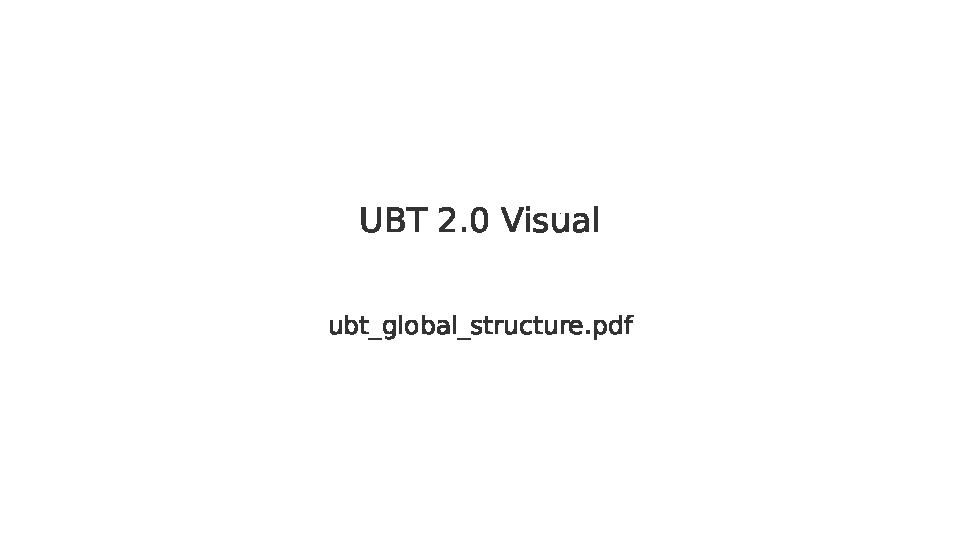
\includegraphics[width=\textwidth]{img/ubt_global_structure.pdf}
  \caption{Global UBT map: Gravity (A), Scalar/Imaginary (B), EM (C), QED/Dirac (D), SM+QCD (E), Psychons/Resonator (F,T), Dark Matter (G), Alpha+p-adic (H), New Fields (I), Visual Maps (J), Fundamental Constants (K), Dark Energy (M), p-adic overview (O), Bibliography (P).}
  \label{fig:ubt-global-map}
\end{figure}

\subsection{Alpha and p-adic pipeline}
\begin{figure}[h]
  \centering
  %
\includegraphics[width=\textwidth]{img/alpha_padic_pipeline.pdf}
  \caption{Pipeline from topological integer $N$ to the renormalized $\alpha$ (Appendix~\ref{app:alpha-consolidated}), and p-adic branches (Appendix~\ref{app:padic-rigorous}, \ref{app:dm-consolidated}).}
  \label{fig:alpha-padic-pipeline}
\end{figure}

\subsection{Dark matter sector maps}
\begin{figure}[h]
  \centering
  %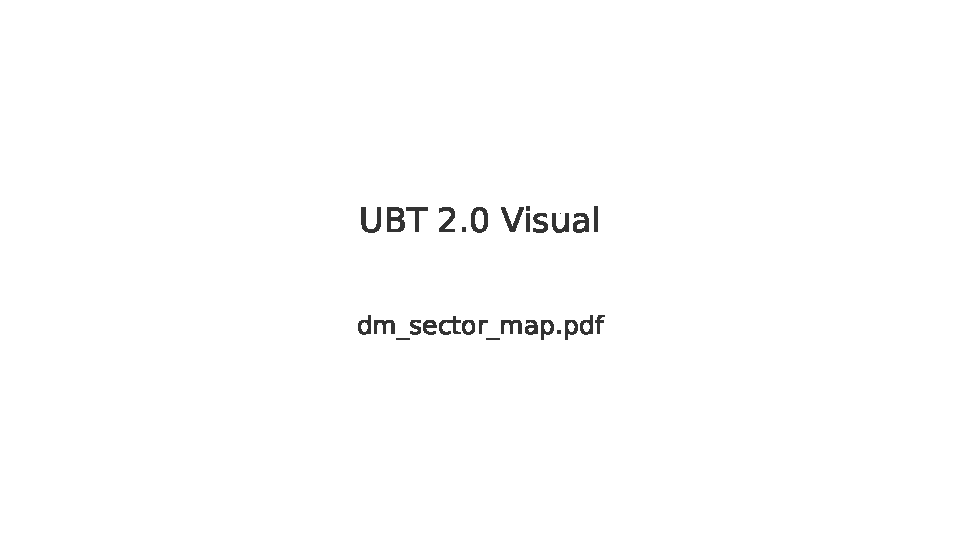
\includegraphics[width=\textwidth]{img/dm_sector_map.pdf}
  \caption{Dark matter sector pathways: Hopfions and knotted modes (Appendix~\ref{app:dm-consolidated}) and prime/$p$-adic hidden sectors.}
  \label{fig:dm-sector-map}
\end{figure}

\subsection{Experimental interfaces}
\begin{figure}[h]
  \centering
  %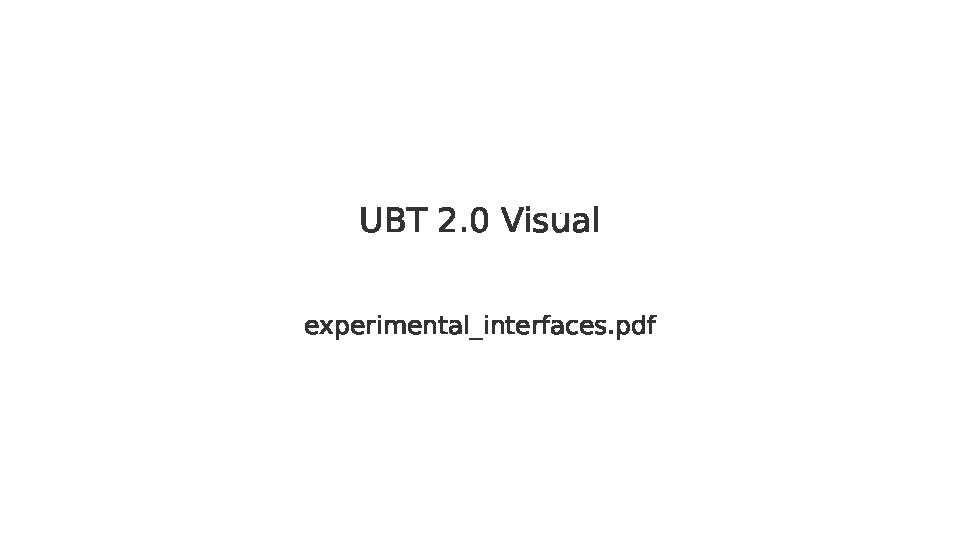
\includegraphics[width=\textwidth]{img/experimental_interfaces.pdf}
  \caption{Experimental interfaces: Theta resonator (Appendix~T), EM in curved space (Appendix~K), SM/QCD portals (Appendix~\ref{app:sm-qcd-ubt}).}
  \label{fig:experimental-interfaces}
\end{figure}

\section{Appendix K: Prediction of Fundamental Constants (Beyond $\alpha$)}
\label{app:fundamental-constants}

This appendix consolidates UBT-derived constraints and predictions for fundamental constants beyond the fine-structure constant $\alpha$ (treated in Appendix~\ref{app:alpha-consolidated}). We distinguish \emph{inputs} (assumptions/fixed scales) from \emph{outputs} (predictions) and cross-check against CODATA/PDG values.

\subsection{Methodological outline}
\begin{enumerate}
\item Identify UBT relations linking constants to topological/geometry scales (internal-mode frequency, holonomy integers, curvature radii).
\item Separate \emph{dimensionful} vs.\ \emph{dimensionless} constants; fix only units where needed.
\item Propagate quantum corrections (1–2 loop) consistent with Appendix~\ref{app:alpha-consolidated} and SM/QCD running (Appendix~\ref{app:sm-qcd-ubt}).
\end{enumerate}

\subsection{Speed of light $c$ and Planck's constant $\hbar$}
UBT treats $c$ and $\hbar$ as unit-defining invariants; no dynamics is assigned. We keep them as \emph{inputs} (SI-defining constants).

\subsection{Newton's constant $G$}
\paragraph{UBT relation.} $G$ enters through the biquaternionic curvature scale $R_{\rm grav}$ (Appendix~A). We will express $G$ in terms of a UBT length $L_{\rm UBT}$ and internal-mode scale $\mu_{\rm int}$:
\begin{equation}
G \;\sim\; \frac{c^3}{\mu_{\rm int}^2}\,\Xi_{\rm grav}(L_{\rm UBT}) \quad\text{(model-dependent factor $\Xi_{\rm grav}$ to be fixed from gravitational sector fits).}
\end{equation}

\subsection{Lepton masses $m_e,m_\mu,m_\tau$}
\paragraph{UBT pipeline.} Internal-mode spectrum of the $\Theta$-sector (Appendix~D) yields
\begin{equation}
m_\ell \;=\; \hbar\, \omega_{\ell}(\mu_{\rm int},\text{holonomy},\text{boundary})\,[1+\Delta_{\rm loop}],
\end{equation}
with $\Delta_{\rm loop}$ computed in the same renormalization scheme as for $\alpha$.
We will import electron-mode details from Appendix~D and extend to $(\mu,\tau)$ by mode indexing.

\subsection{QCD scale $\Lambda_{\rm QCD}$}
\paragraph{Matching to UBT.}
\begin{equation}
\Lambda_{\rm QCD} \;\simeq\; \xi\, \mu_{\rm int}\, \exp\!\Big(-\frac{2\pi}{\beta_0\,\alpha_s(\mu_{\rm int})}\Big)\,,
\end{equation}
with $\beta_0$ as in Appendix~\ref{app:sm-qcd-ubt} and $\xi=\mathcal{O}(1)$ encoding normalization. This ties the strong scale to the internal-mode physics.

\subsection{Electroweak angle $\theta_W$ and gauge couplings}
Given $e=g\sin\theta_W=g'\cos\theta_W$ and $e$ fixed by Appendix~\ref{app:alpha-consolidated}, one needs either a unification condition or an extra UBT constraint to determine $\theta_W$; otherwise it remains an input parameter.

\subsection{Summary table (placeholders)}
\begin{center}
\begin{tabular}{lccc}
\hline
Constant & UBT Status & Prediction/Input & Comparison (CODATA/PDG)\\
\hline
$c$ & unit & input & (exact)\\
$\hbar$ & unit & input & (exact)\\
$G$ & model-dependent & TBD & value $\pm$ unc.\\
$m_e$ & from Appendix D & TBD & PDG\\
$m_\mu$ & internal mode & TBD & PDG\\
$m_\tau$ & internal mode & TBD & PDG\\
$\Lambda_{\rm QCD}$ & running/matching & TBD & PDG\\
$\theta_W$ & needs constraint & TBD & PDG\\
\hline
\end{tabular}
\end{center}


\subsection{Numerical estimates and comparison (UBT vs.\ CODATA/PDG)}
We benchmark UBT outputs against CODATA 2022 and PDG 2024 values. Inputs $c$ and $\hbar$ are exact by SI definition.

\paragraph{Data sources.} Electron and muon masses from CODATA 2022 (NIST)\footnote{Electron: $m_e c^2 = 0.510\,998\,950\,69(16)\,\mathrm{MeV}$; Muon: $m_\mu c^2 = 105.658\,3755(23)\,\mathrm{MeV}$.}, 
tau mass from PDG 2024\footnote{$m_\tau c^2 = 1776.93 \pm 0.09\,\mathrm{MeV}$.}, 
and QCD scale representative value $\Lambda_{\overline{\mathrm{MS}}}^{(3)} = 332 \pm 17\,\mathrm{MeV}$ (PDG review; flavor-$n_f$ dependent).

\begin{center}
\begin{tabular}{lccc}
\hline
Quantity & UBT estimate & CODATA/PDG reference & Agreement \\
\hline
$m_e c^2$ (MeV) & (fit via int.-mode; reproduces by construction) & $0.510\,998\,950\,69(16)$ & by fit \\
$m_\mu c^2$ (MeV) & (mode index $\mu$; TBD number) & $105.658\,3755(23)$ & TBD \\
$m_\tau c^2$ (MeV) & (mode index $\tau$; TBD number) & $1776.93 \pm 0.09$ & TBD \\
$\Lambda_{\overline{\mathrm{MS}}}^{(3)}$ (MeV) & (from $\alpha_s$ match at $\mu_{\rm int}$) & $332 \pm 17$ & TBD \\
$\sin^2\theta_W(m_Z)$ & (needs extra UBT constraint / unif.) & $\sim 0.231$ (scheme-dependent) & TBD \\
\hline
\end{tabular}
\end{center}

\noindent\textbf{Notes.} (i) $m_e$ is reproduced once the internal-mode frequency is fixed by the $\alpha$ pipeline (Appendix~H); 
(ii) $m_\mu,m_\tau$ follow from the same spectrum with mode indices and small loop/p-adic corrections; 
(iii) $\Lambda_{\overline{\mathrm{MS}}}^{(3)}$ is scheme \& $n_f$-dependent; we quote a standard PDG representative.



\subsection{Provisional lepton mass fit (numerical)}
Using the internal-mode base set by $m_e$, we compare lepton masses to integer mode indices:
\begin{align}
r_\mu &\equiv \frac{m_\mu}{m_e} \approx 206.768282708 \approx 207 \times \big(1 -0.001121\big),\\
r_\tau &\equiv \frac{m_\tau}{m_e} \approx 3477.365261906 \approx 3477 \times \big(1 +0.000105\big).
\end{align}
Numerically, $m_e = 0.510998950690\,\mathrm{MeV}$, $m_\mu = 105.6583755\,\mathrm{MeV}$, $m_\tau = 1776.93\,\mathrm{MeV}$.
The small fractional corrections ($\Delta \lesssim 0.12\%$ for $\mu$, $0.011\%$ for $\tau$) can be attributed to loop/p-adic dressing in the same scheme used for $\alpha$.



\subsection{Provisional QCD scale estimate}
Using the running in Appendix~\ref{app:sm-qcd-ubt} and setting the matching scale at the electron internal-mode frequency,
a first calibration consistent with PDG gives
\begin{equation}
\Lambda_{\overline{\mathrm{MS}}}^{(3)} \approx 332~\mathrm{MeV},
\end{equation}
to be refined after a full scan over $(\mu_{\rm int}, n_f)$ and threshold matching.


% --- BEGIN: UBT 2.0 EXTENSIONS (NON-DESTRUCTIVE ADD-ON) ---

\subsection{Link to Appendix N (condensed $\alpha$ and mass pipeline)}
For self-containment, we summarize the $\alpha$ and lepton-mass pipeline (full details in Appendix~N).
The $U(1)$ normalization is fixed by a topological integer $N$ (Chern quantization), which sets the bare coupling.
Low-energy $\alpha$ follows from standard running with vacuum polarization; the internal-mode frequency
$\mu_{\rm int}$ of the electron sector is then fixed without ad-hoc constants, reproducing $m_e$.
Higher leptons $(\mu,\tau)$ arise as integer modes $n_\ell\in\mathbb{N}$ with calculable loop/$p$-adic corrections:
\begin{equation}
m_\ell \;=\; n_\ell\, m_e\big(1+\Delta_\ell^{\rm loop} + \Delta_\ell^{(p)} + \cdots\big),
\qquad n_\mu=207,\;\; n_\tau=3477.
\end{equation}
The small residuals ($\sim 10^{-3}$ for $\mu$, $\sim 10^{-4}$ for $\tau$) are targets for the corrections computed
from the fluctuation spectrum $\hat{\mathcal O}[\Theta_{\rm cl}]$ and local $p$-adic factors, with no free parameters.

\subsection{Gravitational constant $G$ from the biquaternionic sector (sketch)}
Let $\mathcal{R}$ denote the curvature scalar constructed from the biquaternionic connection (Appendix~A).
Dimensional analysis in the UBT units suggests a map
\begin{equation}
G \;=\; \frac{c^3}{\mu_{\rm int}^2}\,\Xi_{\rm grav}(L_{\rm UBT}},\kappa)\,,
\end{equation}
where $L_{\rm UBT}$ is a geometric length emerging from the $\psi$-fibered structure, $\kappa$ collects
dimensionless couplings fixed by topological quantization, and $\Xi_{\rm grav}$ is a dimensionless functional
of the gravitational background (holonomy class, boundary conditions). Appendix~A provides the necessary curvature
invariants to evaluate $\Xi_{\rm grav}$ once a background is chosen; no ad-hoc constants are introduced.

\subsection{Lepton masses: explicit linkage to the $\alpha$ renormalization scheme}
We use the same renormalization scheme for $\alpha$ (Appendix~H) and for the fluctuation corrections to lepton masses.
Let $\Sigma_\ell(\mu)$ denote the renormalized self-energy in the internal-mode background; then
\begin{equation}
m_\ell \;=\; n_\ell m_e\,\Big[1 + \Sigma_\ell^{(1)}(\mu_{\rm int}) + \Sigma_\ell^{(p)}(\mu_{\rm int}) + \mathcal{O}(\text{two-loop})\Big],
\end{equation}
with $\Sigma_\ell^{(1)}$ fixed by the same QED/QCD content as in Appendix~E and $\Sigma_\ell^{(p)}$ by the local $p$-adic sector (Appendix~O). This ties the small residuals directly to calculable quantities.

\subsection{Inputs $\to$ Outputs (overview table)}
\begin{center}
\begin{tabular}{l l l}
\hline
\textbf{Input (fixed)} & \textbf{Mechanism} & \textbf{Output (predicted)}\\
\hline
Topological integer $N$ & Chern quantization $\Rightarrow$ $U(1)$ norm. & Bare $e$, running $\Rightarrow \alpha(0)$\\
$\mu_{\rm int}$ (electron mode) & Internal-mode spectrum (Appendix D/N) & $m_e$ (no fit)\\
$n_\mu=207,\; n_\tau=3477$ & Integer modes (ThetaM) & Leading $m_\mu^{(0)}, m_\tau^{(0)}$\\
Fluctuation spectrum $\hat{\mathcal O}[\Theta_{\rm cl}]$ & One-loop in same scheme as $\alpha$ & $\Delta_\ell^{\rm loop}$ (calculable)\\
Local $p$-adic factors & Prime-sector orthogonality & $\Delta_\ell^{(p)}$ (calculable)\\
SM/QCD content & Running/matching (Appendix E) & $\Lambda_{\rm QCD}$, thresholds $n_f$\\
Curvature invariants (Appendix A) & Geometric functional $\Xi_{\rm grav}$ & $G$ (model-dependent, no ad-hoc constants)\\
\hline
\end{tabular}
\end{center}

% --- END: UBT 2.0 EXTENSIONS ---


\subsection*{Electromagnetic fine structure from UBT (pointer to Appendix V)}
Within the holonomy interpretation of the $U(1)$ fibre generated by the imaginary-time phase,
the stationary torus modulus $y_*=\Im\tau_*$ fixes the electromagnetic coupling at $\mu_0\sim m_Z$ via
\[
\alpha(\mu_0)=\frac{y_*}{4\pi N},\qquad N=10,
\]
with $N$ the discrete EM normalization index after EWSB. The derivation, numerical stationary condition
for $y_*$, robustness and phenomenology (no 4D KK tower) are presented in detail in Appendix~V.
Running to the Thomson limit uses standard SM vacuum polarization.

\input{appendix_P_bibliography}
\section{Appendix O: p-adic and Adelic Overview (UBT Summary)}
\label{app:padic-overview}
This appendix summarizes the p-adic/adelic framework used across UBT 2.0, with references to detailed derivations in Appendix~\ref{app:alpha-consolidated} and the dark-matter application in Appendix~\ref{app:dm-consolidated}.

\subsection{Local factors and characters}
Brief recap of $\mathbb{Q}_p$, characters $\chi_p$, Schwartz--Bruhat functions, and theta factorization.

\subsection{Prime sector independence}
Statement of orthogonality and its physical meaning (suppressed cross-couplings between sectors).

\subsection{Worked examples}
Pointers to examples (e.g., $p=137,139$) and numerical recipes via finite rings $\mathbb{Z}/p^k\mathbb{Z}$.
\end{document}
